\documentclass[main.tex]{subfiles}
\begin{document}
处理字的符的 Python 程序

\begin{figure}
	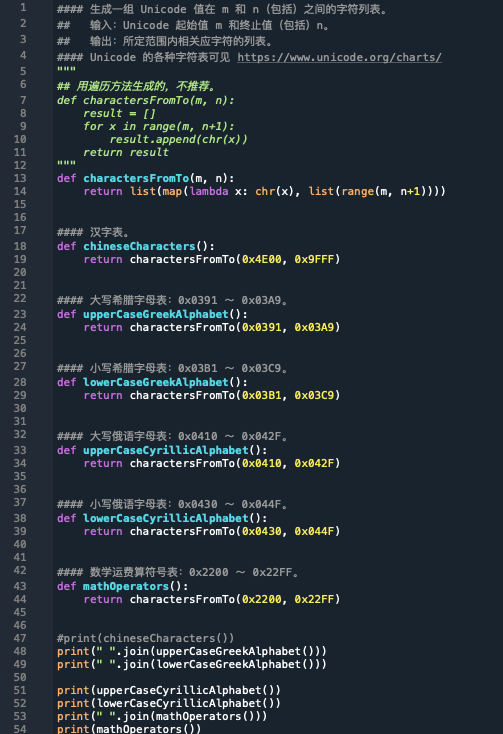
\includegraphics{string.png}
\end{figure}

Python 程序 xxx 生成希腊的字母如下:


从 Unicode 表中 Python 程序 xxx 生成部分常用数学运算速度符号如果下:

\newpage
\begin{figure}
	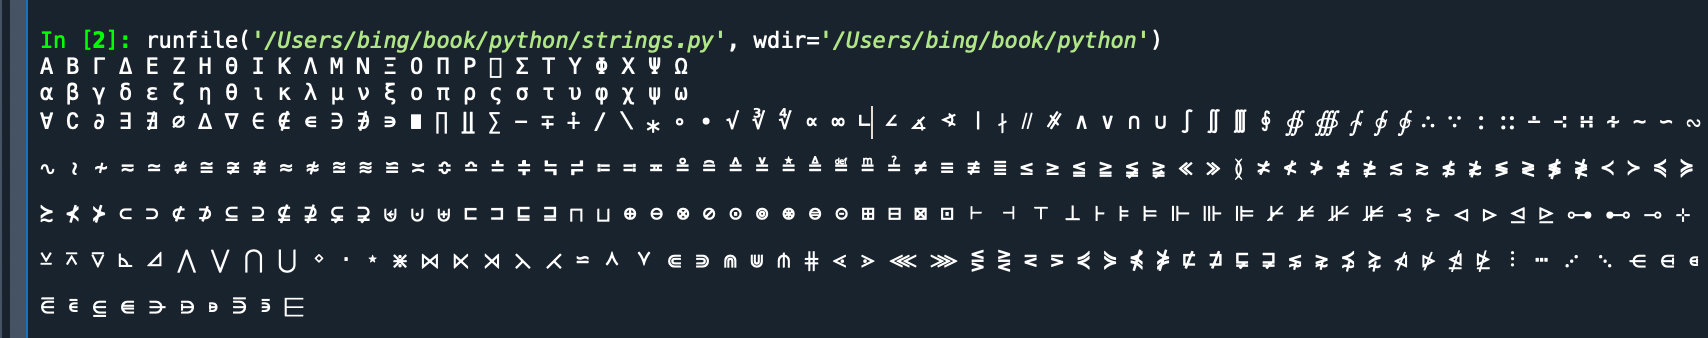
\includegraphics{greek_math_symbols.png}
\end{figure}


字符串处理
华罗庚数论导引
\cite[p.~1]{华罗庚数论导引}

钟尔杰数学实验方法 \cite{钟尔杰数学实验方法}

钟尔杰数值分析讲义 \cite{钟尔杰数值分析讲义}

\newpage
\end{document} 